% begin module polar-intro
\begin{frame}[t]
\frametitle{Polar Coordinates}
\begin{itemize}
\item<1->  The polar coordinate system is an alternative to the Cartesian coordinate system.
%\item  Instead of specifying horizontal distance and vertical distance, we specify angle and distance from the origin.
\item<2-> Choose a point in the plane called $O$ (the origin).
\item<3-> Draw a ray starting at $O$. The ray is called the polar axis.  This ray is usually drawn horizontally to the right.
\end{itemize}
\begin{columns}[c]
\column{.5\textwidth}
\psset{xunit=5cm, yunit=5cm}
\begin{pspicture}(-0.2, -0.2)(1.500000,0.6)
\tiny
%force a boudning box:
\psline[linecolor=red!1](-0.1, -0.1)(-0.21,0.2)
\psline[linecolor=red!1](1.1, 0.6)(1.1,0.61)

\uncover<5->{
%Calculator input: plotCurve{}(1/5 \cos{}t, 1/5 \sin{}t, 0, 1/6 \pi)
\parametricplot[arrows=->, linecolor=red, plotpoints=1000] {0}{0.523599}{t 57.29578 mul cos 0.2 mul t 57.29578 mul sin 0.2 mul }
\psline[linecolor=blue](0,0)(0.866025404, 0.5)
\rput(0.22, 0.06){$\alert<5>{\theta}$}
}

\uncover<4->{
\fcFullDotBlue{0.866025404}{0.5}
\rput[l](0.88, 0.5){$P\uncover<7->{\alert<7>{(r,\theta)}}$}
}

\uncover<2->{
\fcFullDotBlue{0}{0}
\rput(-0.1, 0){$O$}
}
\uncover<6->{
\rput(0.4, 0.3){$\alert<6>{r}$}
}
\uncover<3->{
\psline{->}(0,0)(1,0)
\rput (0.5, -0.05){polar axis}
}
\end{pspicture}

\vspace{1cm}

%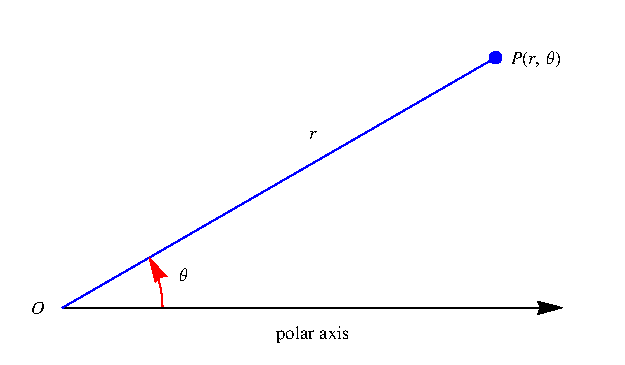
\includegraphics[height=4cm]{polar-curves/pictures/11-03-polar.pdf}%
\column{.5\textwidth}
\begin{itemize}
\only<1-7>{\item<4->  Let $P$ be a point in the plane.
\item<5-> Let $\theta$ denote the angle between the polar axis and the line $OP$.
\item<6-> Let $r$ denote the length of the segment $OP$.
\item<7-> Then $P$ is represented by the ordered pair $(r, \theta )$.
}
\only<8->{
\item<8-> The letters $(x,y)$ imply Cartesian coordinates and the letters $(r, \theta)$- polar. \uncover<9->{When we use other letters, it should be clear from context whether we mean Cartesian or polar coordinates.} \uncover<10->{If not, one must request clarification.}
}
\end{itemize}
\end{columns}
\end{frame}
% end module polar-intro
